\documentclass[tikz]{standalone}
\usepackage[T1]{fontenc}
\usepackage[utf8]{inputenc}
\usepackage{tikz,pgfplots}
\usepackage{grffile}
\pgfplotsset{compat=newest}
\usetikzlibrary{plotmarks,positioning,fit,shapes.geometric,arrows,external,matrix,backgrounds,spy}
\usepgfplotslibrary{patchplots,groupplots,statistics}
\usepackage{siunitx,xcolor,physics}
\usepackage{sfmath}
\renewcommand{\familydefault}{\sfdefault}
\newcommand{\mat}[1]{\mathbf{#1}}

\begin{document}

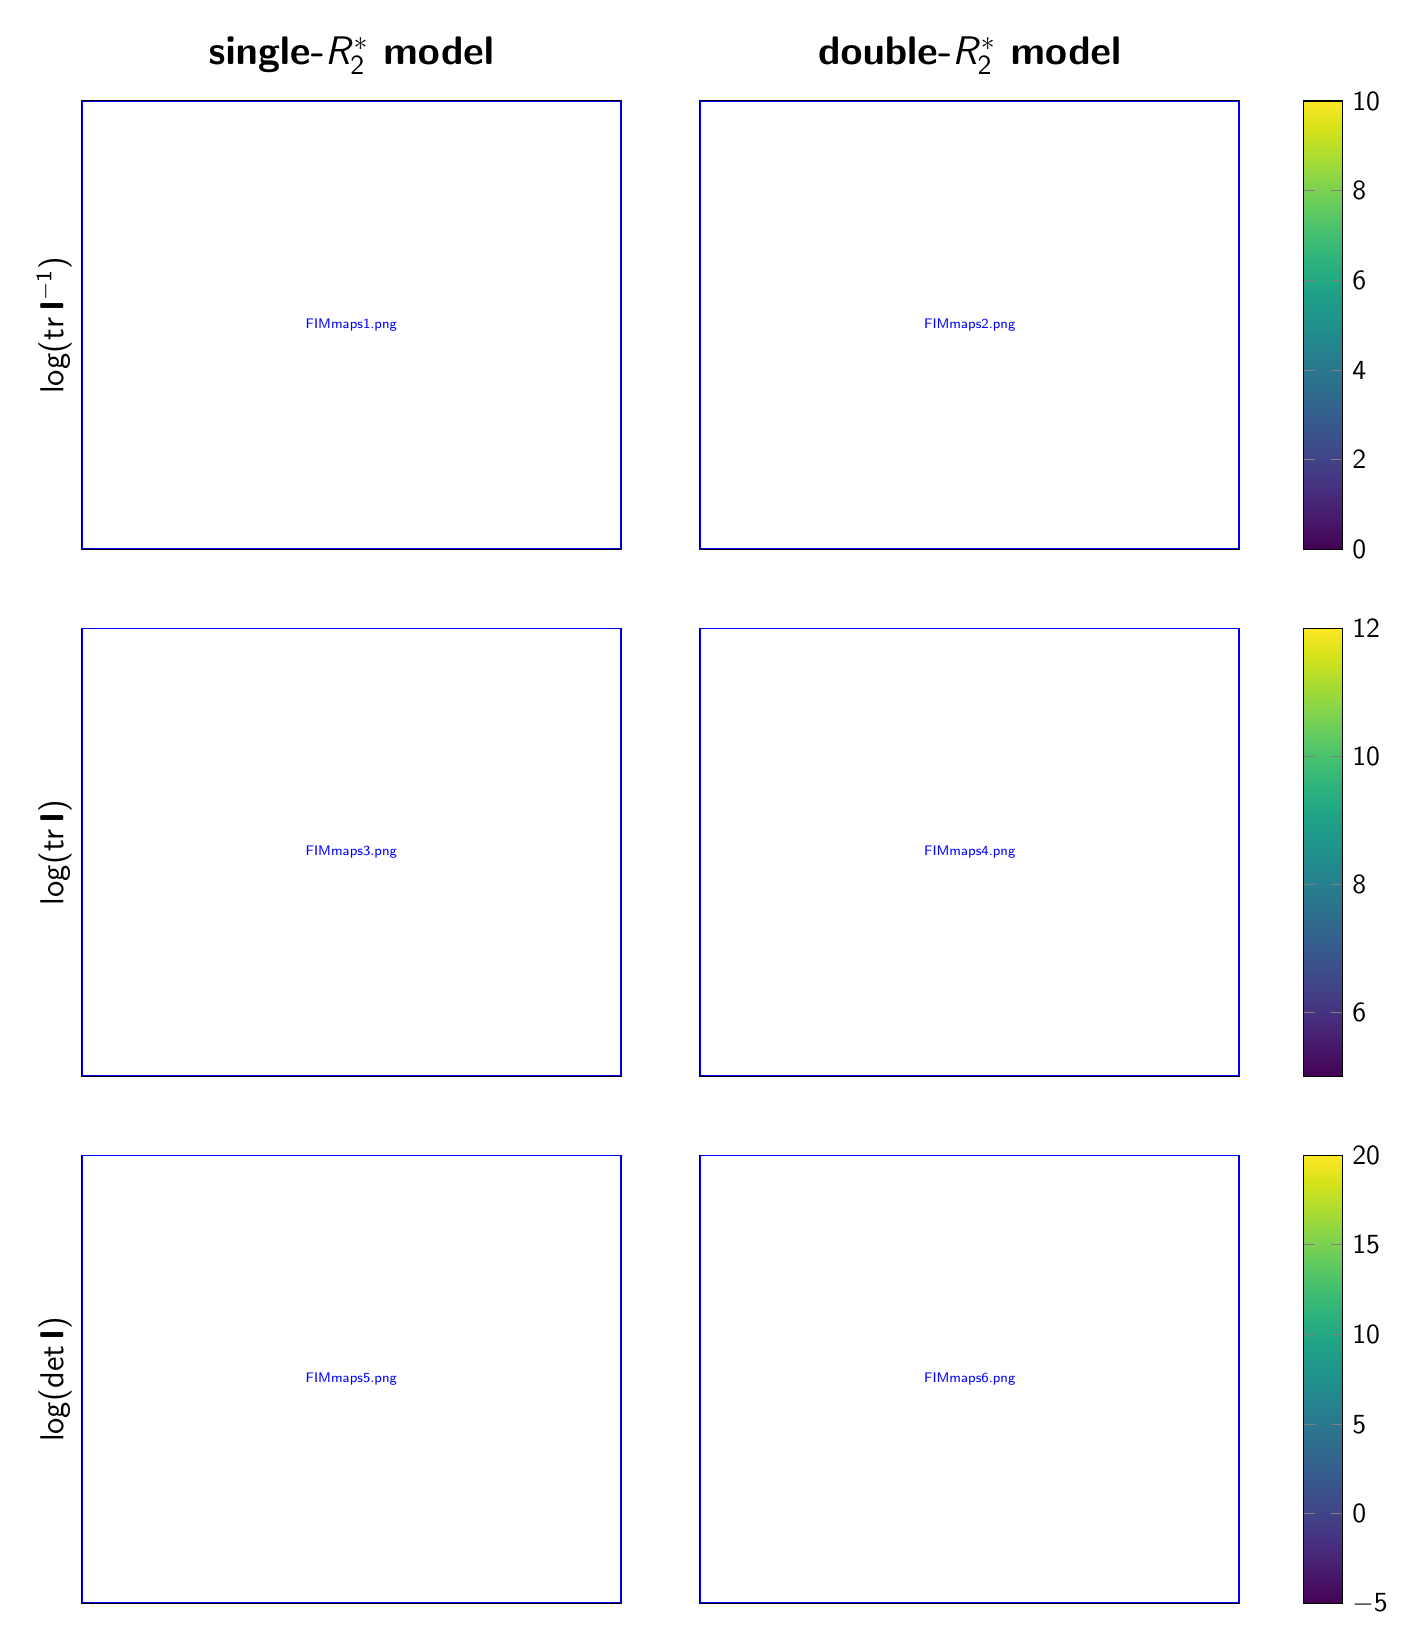
\begin{tikzpicture}
  \pgfplotsset{every axis plot/.append style={line width=4.pt}}
  \pgfplotsset{
    % tick label style = {font=\sansmath\sffamily},
    % every axis label = {font=\sansmath\sffamily},
    % legend style = {font=\sansmath\sffamily},
    title style={font=\large},
    label style = {font=\large}
  }

  \begin{groupplot}[%
    group style={group size=2 by 3,
      horizontal sep=1cm,
      vertical sep=1cm,
    },
    xmin=-0.5, xmax=223.5,
    ymin=-0.5, ymax=223.5,
    xtick=\empty,
    ytick=\empty,
    % colorbar,
    colormap/viridis,
    colorbar style={xshift=0.5cm}
    ]


    \nextgroupplot[
    point meta min=0,
    point meta max=10,
    title={\bf\Large single-\(R_2^{*}\) model},
    ylabel={$\log(\tr \mat{I}^{-1})$},
    ]

    \addplot graphics [includegraphics cmd=\pgfimage,xmin=-0.5, xmax=223.5, ymin=223.5, ymax=-0.5] {FIMmaps1.png};


    \nextgroupplot[
    point meta min=0,
    point meta max=10,
    colorbar,
    title={\bf\Large double-\(R_2^{*}\) model},
    ]

    \addplot graphics [includegraphics cmd=\pgfimage,xmin=-0.5, xmax=223.5, ymin=223.5, ymax=-0.5] {FIMmaps2.png};


    \nextgroupplot[
    point meta min=5,
    point meta max=12,
    ylabel={$\log(\tr \mat{I})$},
    ]

    \addplot graphics [includegraphics cmd=\pgfimage,xmin=-0.5, xmax=223.5, ymin=223.5, ymax=-0.5] {FIMmaps3.png};


    \nextgroupplot[
    point meta min=5,
    point meta max=12,
    colorbar,
    ]

    \addplot graphics [includegraphics cmd=\pgfimage,xmin=-0.5, xmax=223.5, ymin=223.5, ymax=-0.5] {FIMmaps4.png};


    \nextgroupplot[
    point meta min=-5,
    point meta max=20,
    ylabel={$\log(\det \mat{I})$},
    ]

    \addplot graphics [includegraphics cmd=\pgfimage,xmin=-0.5, xmax=223.5, ymin=223.5, ymax=-0.5] {FIMmaps5.png};


    \nextgroupplot[
    point meta min=-5,
    point meta max=20,
    colorbar,
    ]

    \addplot graphics [includegraphics cmd=\pgfimage,xmin=-0.5, xmax=223.5, ymin=223.5, ymax=-0.5] {FIMmaps6.png};



\end{groupplot}

\end{tikzpicture}


\end{document}